%%% Local Variables:
%%% mode: latex
%%% TeX-master: "report_main"
%%% End:

\section{Part 1 - Mathematical modeling}
\subsection{Problem 1}

We use the helicopter model \cref{fig:helicopter_model} as our
starting point for deriving the equations of motion.

\begin{figure}[hbp]
  \caption{the helicopter model figure 7 from the assignment
    \cite[p.12]{assignment} with relevant distances drawn in.}

  \label{fig:helicopter_model}
  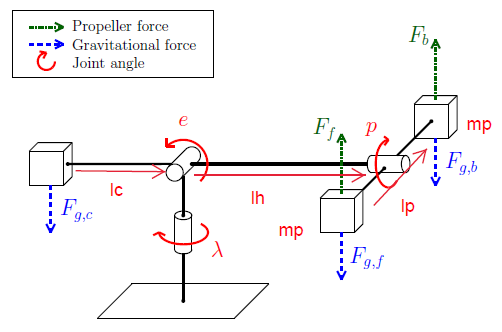
\includegraphics[width=\textwidth]{images/helicopter_model}
\end{figure}

The equation of motion for the pitch is found through the momentum
around the pitch axis in the clockwise direction as shown in
\cref{fig:helicopter_model}. It becomes:

\begin{align*}
  J_p\ddot{p} &= l_p(F_{g,b} - F_b - F_{g,f} + F_f) \\
              &= l_p(m_pg - mp_g + K_fV_f - V_b) \\
              &= l_pK_f(V_f-V_b)
\end{align*}
Since $V_d = V_f-V_b$, we can write this as:
\begin{equation}
  J_p\ddot{p} = l_pK_fVd
\end{equation}
Here, we can see that $L_1 = l_pK_f$.

The equation of motion for the elevation angle is found similarly
through the momentum in the counter-clockwise direction around the
elevation axis.

\begin{align*}
  J_e\ddot{e} &= arm_cF_{g,c} - arm_h(F_{g,f}+F_{g_b} - K_fcos(p)(V_f + V_b))
\end{align*}
where $arm_c$ is the moment arm between the counterweight point mass
and the elevation axis, and $arm_h$ is the moment arm between any of
the two motor point masses and the elevation axis. As shown in
\cref{fig:elevation_model}, $arm_c = l_ccos(e)$, and $arm_h =
l_hcos(e)$. \todo{Husk at figuren må være som jeg (Daniel) har i
  notatene her, da er det 100 prosent tydelig hva $arm_c$ og $arm_h$
  blir. Kan godt gjøre det enda litt mer detaljert.} We can
immediately substitute $V_s = V_f + V_b$, and simplify:

\begin{align*}
  J_e\ddot{e} &= l_ccos(e)m_cg - l_hcos(e)(2m_pg - K_fcos(p)V_s) \\
              &= cos(e)(l_cm_cg - 2l_hm_pg) + l_hK_fV_scos(e)cos(p)
\end{align*}
Here, we have (as the author of the exercise) counted the cos(e)
factor of the $V_s$ term as negligible, and set it to 1. \todo{Forklar
  hvor cos(p) kommer fra - og lag ny figur. Bruk denne til å forklare
  (2c)/(3) også.} The resulting equation has the form:

\begin{equation}
  J_e\ddot{e} = g(l_cm_c - 2l_hm_p)cos(e) + l_hK_fV_scos(p)
\end{equation}
Note that $L_2 = g(l_cm_c-2l_hm_p)$, and $L_3 = l_hK_f$.

\begin{figure}[H]
  \caption{the elevation model}
  \label{fig:elevation_model}
  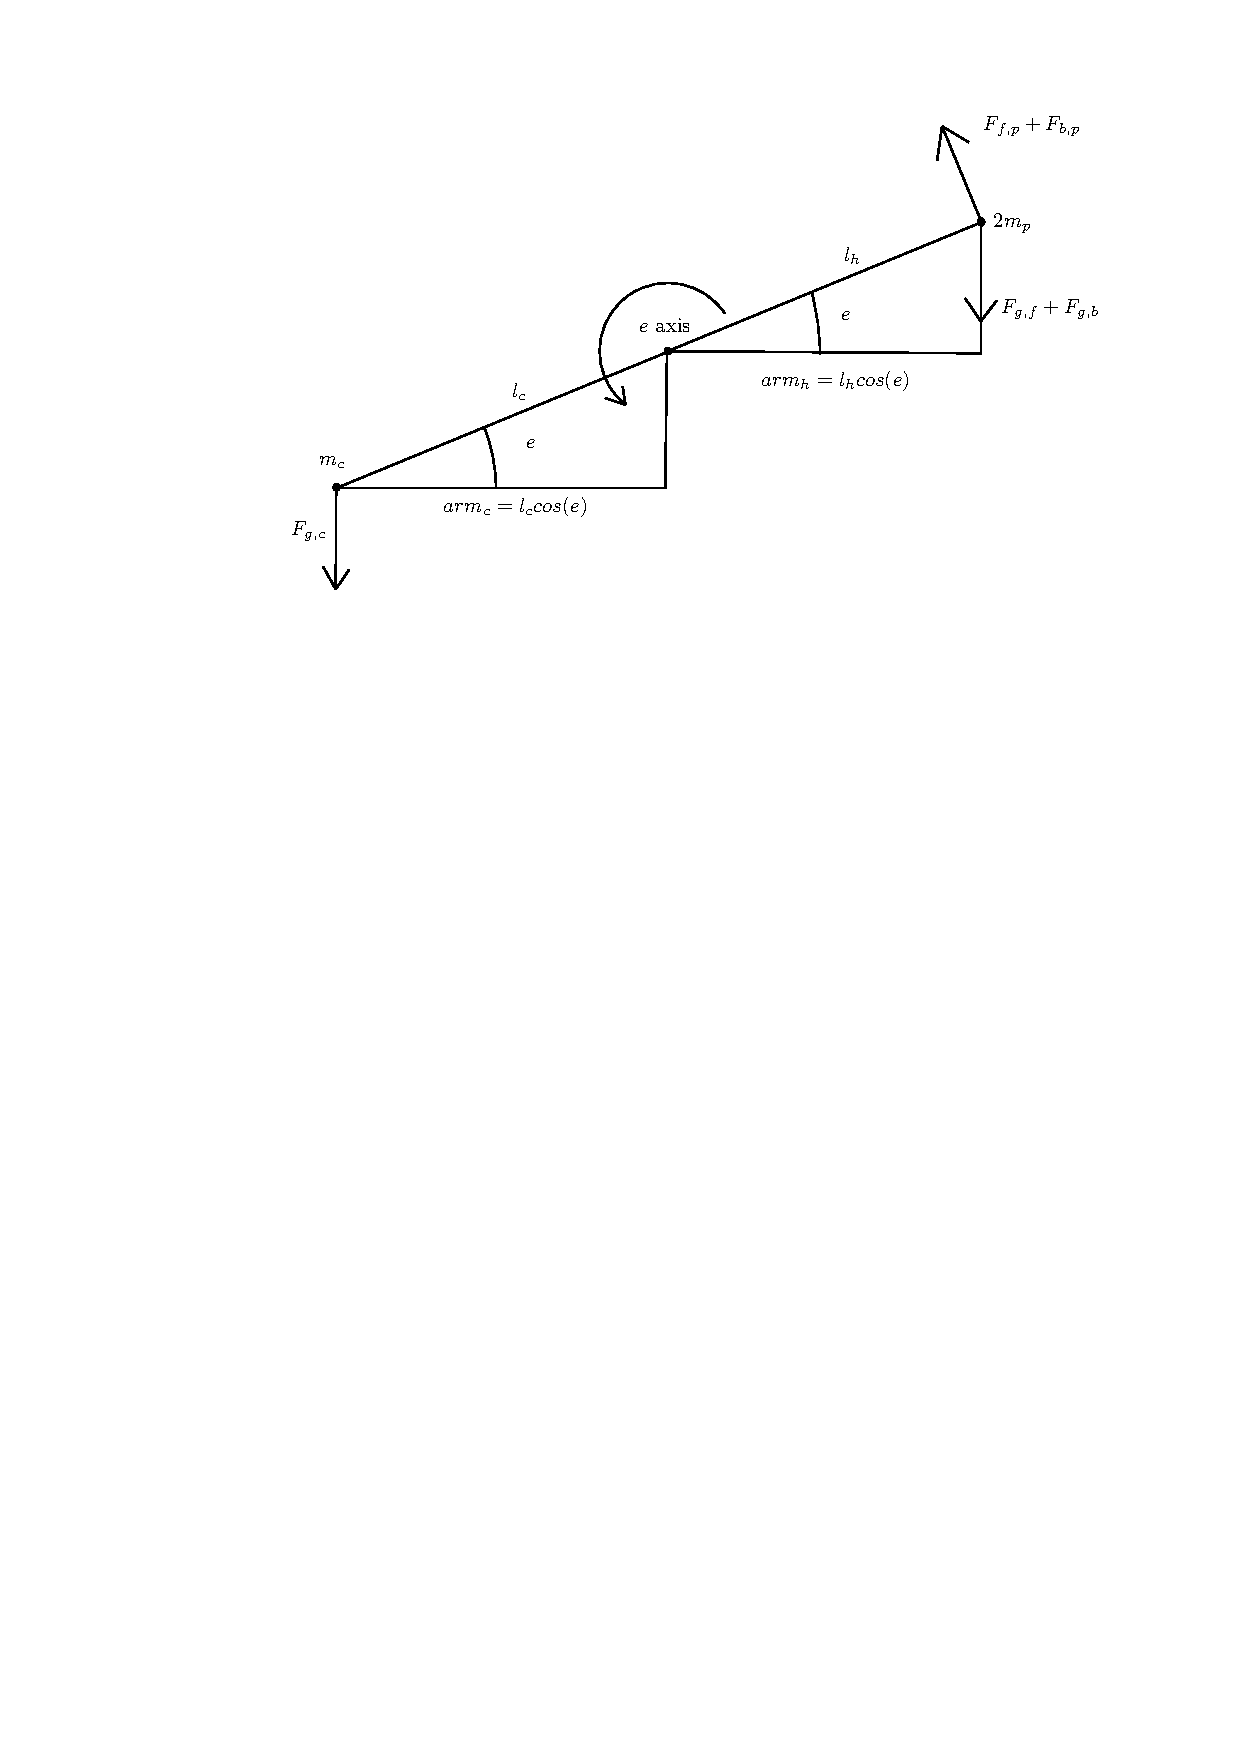
\includegraphics[width=0.5\textwidth]{images/elevation_model}
\end{figure}

Finally, the equation of motion for the travel angle is found through
the momentum around the travel axis in the  clockwise direction. As
seen in \cref{fig:elevation_model}, the only forces with a moment arm
perpendicular to the travel axis are the components of the motor
forces in the horizontal direction, which have length $arm_h =
l_hcos(e)$. Furthermore, the horizontal components


\begin{figure}[H]
  \caption{the pitch model}
  \label{fig:pitch_model}
  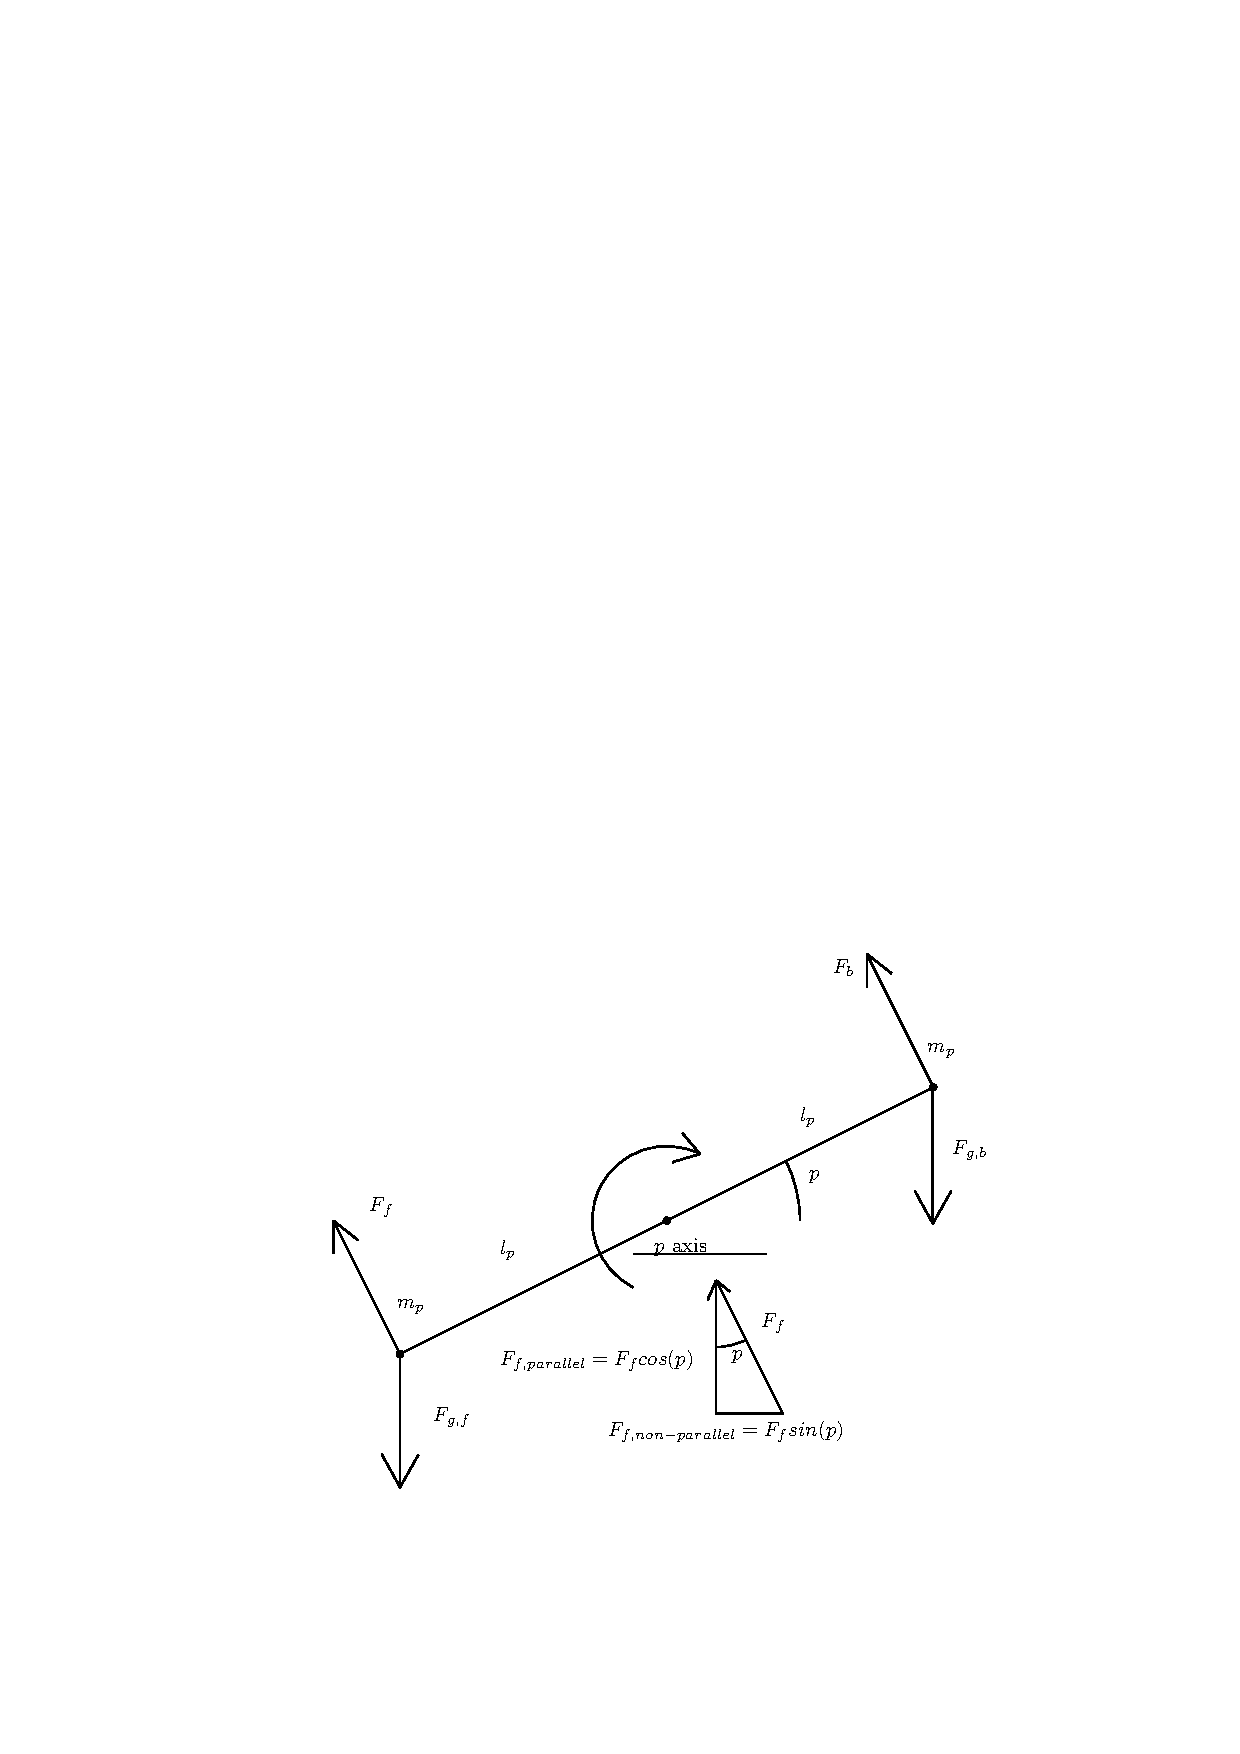
\includegraphics[width=0.5\textwidth]{images/pitch_model}
\end{figure}

\begin{align*}
  J_\lambda\ddot{\lambda} &= arm_h
\end{align*}

The equations (1), (2), and (3) corresponds to (2a), (2b), and (2c) respectively of the assignment \cite[p.13]{assignment}

\subsection{Problem 2}
To linearize the system about the point with all state variables equal
to zero $(p, e, \lambda)^T = \dot{p},(\dot{e},\dot{\lambda}=^T $ = (0, 0, 0))
the inputs in the equations of motion ($V^{*}_{s} \text{and} V^{*}_{d}$) must be set to
values that make this an equilibrium point.

At the linearization point, the equation of motion for pitch
(\todo{ADD EQUATION REFERENCE}) reduces to $0 = L_{1} *
V^{*}_{d}$ therefore
:
\begin{equation}
  V^{*}_{d} = 0
\end{equation}
At the linearization point, the equation of motion for elevation
(\todo{ADD EQUATION REFERENCE}) reduces to $0 = L_{2} +
L_{3}*V^{*}_{s}$ therefore:

\begin{equation}
  V^{*}_{s} = -L_{2} / L_{3}
\end{equation}
While the equation of motion for travel (\todo{ADD EQUATION
  REFERENCE}) at the linearization point simply reduces to 0 = 0.\\
The following transformation is performed to simplify the analysis
\todo{Add cite of assignment here}:

\begin{equation}
  \begin{bmatrix}
    \tilde{p} \\
    \tilde{e} \\
    \tilde{\lambda}
  \end{bmatrix}
  =
  \begin{bmatrix}
    p \\
    e \\
    \lambda
  \end{bmatrix}
  -
  \begin{bmatrix}
    p^{*} \\
    e^{*} \\
    \lambda^{*}
  \end{bmatrix}
  and
  \begin{bmatrix}
    \tilde{V}_{s} \\
    \tilde{V}_{d}
  \end{bmatrix}
  =
  \begin{bmatrix}
    V_{s} \\
    V_{d}
  \end{bmatrix}
  -
  \begin{bmatrix}
    V^{*}_{s} \\
    V^{*}_{d}
  \end{bmatrix}
\end{equation}
The equations of motion in the transformed system are therefore:
\begin{subequations}
  \begin{align}
    J_p\ddot{\tilde{p}} &= L_1\tilde{V_d} \\
    J_e\ddot{\tilde{e}} &= L_2cos(\tilde{e}) + L_3(\tilde{V_s}+L_2/L_3)cos(\tilde{p}) \\
    J_{\lambda}\ddot{\tilde{\lambda}} &= L_4(\tilde{V_s}+L_2/L_3)cos(\tilde{e})sin(\tilde{p})
  \end{align}
\end{subequations}
By choosing the state to be x = ($\tilde{p}$, $\tilde{e}$,
$\tilde{\lambda}$, \textit{$\dot{p}$, $\dot{e}$,$\dot{\lambda}$}) the
nonlinear state equations become:

\begin{subequations}
  \begin{align}
    \dot{x}_1 &= x_4 \\
    \dot{x}_2 &= x_5 \\
    \dot{x}_3 &= x_6 \\
    \dot{x}_4 &= (L_1/J_p) V_d \\
    \dot{x}_5 &= (L_2/J_e)cos(x_2) + (L_3/J_e)(V_s + L_2 / L_3)cos(x_1) \\
    \dot{x}_6 &= (L_4 / J_\lambda) (V_s + L_2 / L_3)cos(x_2)sin(x_1)
  \end{align}
\end{subequations}
If the above system is expressed as $\dot{x} = h(x, u)$, where x is
the state and u is the input, the system is linearized by finding the
Jacobians of h with respect to the state and the input and then
plugging in the equilibrium values.

\begin{equation}
  \frac{\partial h}{\partial x} = A =
  \begin{bmatrix}
    0 & 0 & 0 & 1 & 0 & 0 \\
    0 & 0 & 0 & 0 & 1 & 0 \\
    0 & 0 & 0 & 0 & 0 & 1 \\
    0 & 0 & 0 & 0 & 0 & 0 \\
    0 & 0 & 0 & 0 & 0 & 0 \\
    \frac{L_4L_2}{J_\lambda L_3} & 0 & 0 & 0 & 0 & 0
  \end{bmatrix}
  \qquad
  \frac{\partial h}{\partial u} = B =
  \begin{bmatrix}
    0 & 0 \\
    0 & 0 \\
    0 & 0 \\
    0 & L_1/J_p \\
    L_3/J_e & 0 \\
    0 & 0
  \end{bmatrix}
\end{equation}
where $L_1, L_2, L_3$ and $L_4$ were calculated in Section 1.1
\todo{maybe cite this} and $J_p, J_e$ and $J_\lambda$ were given in
the assignment description \todo{add cite to assignment}.

The linearized equations of motion can therefore be written in the
following form:

\begin{subequations}
  \begin{align}
    \ddot{\tilde{p}} &= K_1\tilde{V}_d \qquad K_1 = \frac{L_1}{J_p}\\
    \ddot{\tilde{e}} &= K_2\tilde{V}_s \qquad K_2 = \frac{L_3}{J_e}\\
    \ddot{\tilde{\lambda}} &= K_3\tilde{p} \qquad K_2 = \frac{L_4L_2}{J_\lambda L_3}
  \end{align}
\end{subequations}
\subsection{Problem 3}
\subsection{Problem 4}

%%% Local Variables:
%%% mode: latex
%%% TeX-master: "report_main"
%%% End:
